% !TEX root = ../00_thesis.tex

\section{Overview of \DRP}
\label{sec:design_overview}

\afterpage{
\begin{figure}
  \centering
  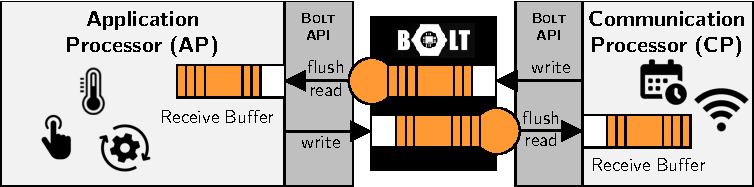
\includegraphics[scale=1]{dpp}
  \caption{Conceptual view of the DPP, based one the \bolt processor interconnect. %
  \capt{%
    Using functions \emph{\opwrite}, \emph{\opread}, and \emph{\opflush}, the application (\ap) and communication (\cp) processors can asynchronously exchange messages with predictable latency.
    The \AP executes application tasks (\eg sensing, actuation, control, \etc) while the \CP is dedicated to radio communication.}}
  \label{fig:bolt_logical}
\end{figure}
}

This chapter presents the \DRPLong (\DRP), a solution to provide end-to-end real-time guarantees between distributed applications.
Before delving into details, this section provides an overview of \DRP's principles.

The system model of \DRP divides the end-to-end communication between local and wireless parts~(\cref{fig:DRP_sysmodel}):
\begin{description}
  \item[\AP  $\boldsymbol{\leftrightarrow}$ \CP]
  Applications run on dedicated application processors (\APs) which are isolated from the rest of the network by their attached communication processor (\CP).
  Local communication between \APs and \CPs  takes place over the \bolt interconnect~\cite{sutton2015Bolt}, which provides asynchronous message passing with bounded delays.
  This device architecture, called the Dual-Processor Platform (\DPP), is illustrated in \cref{fig:bolt_logical} (more details in \cref{ch:introduction}).

  \item[\CP  $\boldsymbol{\leftrightarrow}$ \CP]
  The \CPs exchange messages over a multi-hop wireless network using the \blink real-time protocol~\cite{zimmerling2017Blink}.
  \blink is adaptive to dynamic changes in traffic demands, energy efficient, and delivers messages in real-time.
\end{description}

The \DPP and \blink are key building blocks to fulfill the \feature{Reliability}, \feature{Adaptability}, \feature{Composability}, and \feature{Efficiency} requirements.
However, two major issues remain in order to achieve \feature{Timeliness}.

First, the communication between \APs and \CPs cannot be completely asynchronous: to guarantee end-to-end deadlines, both processors must look for incoming messages with some minimal rate.
%
Second, \blink assumes a periodic release of messages at the network interfaces (\ie the \CPs); since our flow model is not periodic but sporadic with jitter~(\cref{sec:problem}), messages may be delayed in \CPs buffer until they can be transmitted over the network.

\DRP strikes a balance between  \feature{Composability} and \feature{Efficiency}; that is, between
\begin{itemize}
  \item decoupling the execution of \APs, \CPs, and Blink, and
  \item supporting short the end-to-end deadlines between the \APs.
\end{itemize}
The idea behind \DRP is to split the responsibility of meeting end-to-end deadlines between (i)~the source node $n^s_i$ and \blink, and (ii)~the destination node $n^d_i$;
If the source does not write too many messages, \blink guarantees every message will meet a given network deadline $D$, in turns, the destination commits to read its \bolt queue sufficiently often to meet the flow's end-to-end deadlines \deadlineany.

\DRP formalizes these ``commitments'' into \emph{contracts} between the different entities. The challenge is to define, given the current network state and an end-to-end deadline \deadlineany to satisfy, what must be
% \begin{itemize}
  % \item
  (i)~the network deadline $D$ requested to \blink and
  % \item
  (ii)~the minimal reading rate at the destination node.
% \end{itemize}
The goal is to make these contracts minimally restrictive, such that \APs, \CPs, and Blink can operate as much as possible independently from each other (\feature{Composability}).
